\section{Advanced Tutorials}

This section outlines some of the more advanced features of cylc along with
links to tutorials on these features on the rose documentation website.


\subsection{Advanced Cycling}
\label{advanced-cycling}

So far we have defined cycling using graph section headings of the form
\lstinline{[[[TXX]]]} as in the following example:

\begin{lstlisting}
[scheduling]
    initial cycle point = 2000-01-01T00
    [[dependencies]]
        [[[T00]]]  # Run every day at 00:00
            graph = foo => bar
\end{lstlisting}

This is the simplest form of graph section heading. More powerful forms exist
to help define complex recurrences.

They all follow abbreviations of a basic format - \lstinline{Rn/DATE-TIME/REPEAT_INTERVAL}, an ISO 8601\footnote{\url{https://en.wikipedia.org/wiki/ISO_8601}} recurrence format, where \lstinline{n} is an optional limit on repetitions, \lstinline{DATE-TIME} is a starting date-time, and \lstinline{REPEAT_INTERVAL} is the duration between successive recurrences.

A date-time without a repeat interval must have a missing unit of date or time to extrapolate a repeat interval from. \lstinline{T00} above is short for \lstinline{2000-01-01T00}, and the absence of higher-level day information is taken to mean 'daily'. It is thereforce ultimately short for \lstinline{R/2000-01-01T00/P1D}. This means: starting at \lstinline{2000-01-01T00:00:00}, repeat every day (\lstinline{P1D}) indefinitely (\lstinline{R} with no number limit suffix).

\lstinline{T12} would mean the same thing but starting at \lstinline{2000-01-01T12:00:00}. Another example - \lstinline{01T00} - has missing month information, so it is taken to mean 'monthly' or \lstinline{R/2000-01-01T00/P1M}.

A repeat interval without a date-time is taken to use the initial cycle point as the start date-time. \lstinline{P2D} is taken to mean \lstinline{R/2000-01-01T00/P2D}.

A single \lstinline{R1} is taken to mean 'run once at the initial cycle point'.

\paragraph*{Examples} $ $

\begin{tabular}{l l}
\begin{lstlisting}
[[[ T06, T1845 ]]]
\end{lstlisting}
& Run every day at 06:00 and 18:45\\
\begin{lstlisting}
[[[ 01T00 ]]]
\end{lstlisting}
& Run every month on the first of the month \\
\begin{lstlisting}
[[[ PT15M ]]]
\end{lstlisting}
& Run every 5 minutes \\
\begin{lstlisting}
[[[ +P5D/P1M ]]]
\end{lstlisting}
& Run every month, starting 5 days after the initial cycle point \\
\begin{lstlisting}
[[[ R3/T06 ]]]
\end{lstlisting}
& Run three times, once every day at 06:00
\\
\end{tabular}

\begin{shaded*}
\textbf{Tutorial}: TODO: Link to cylc documentation once next version has gone live
\end{shaded*}


\subsection{Advanced Dependencies}

The \& symbol can be used to condense multiple graph lines, for instance the
following example:

\begin{lstlisting}
graph = """
    foo => bar
    foo => baz
"""
\end{lstlisting}

... can be condensed to \lstinline{graph = foo => bar & baz}.
Graph lines can also be written with the \textbar \, symbol meaning or, for
example in the following example \lstinline{baz} will run as soon as either
\lstinline{foo} or \lstinline{bar} succeed.

\begin{lstlisting}
graph = foo | bar => baz
\end{lstlisting}

Up until now we have written dependencies in the form \lstinline{foo => bar}
which means \lstinline{bar} will trigger (run) as soon as \lstinline{foo}
succeeds. It is possible to trigger tasks off of other states e.g:

\begin{tabular}{ll}
\lstinline[mathescape]=foo:fail $=$> bar= &
\lstinline=bar= triggers if \lstinline=foo= fails \\
\lstinline[mathescape]=foo:submit $=$> bar= &
\lstinline=bar= triggers once \lstinline=foo= has submitted \\
\lstinline[mathescape]=foo:start $=$> bar= &
\lstinline=bar= triggers once \lstinline=foo= starts executing \\
\lstinline[mathescape]=foo:finish $=$> bar= &
\lstinline=bar= triggers once \lstinline=foo= succeeds or fails \\
\end{tabular}


\subsection{Families}
\label{Families}

Often a suite will contain a collection of similar tasks. With cylc these
tasks can be grouped together for convenience. This can be used to factor out a lot of repeated configuration to make suites more readable and maintainable.

\paragraph*{Example}
In the following example the
task \lstinline{hello_eris} inherits the \lstinline{script} setting and
\lstinline{IS_WORLD_A_PLANET} environment variable from the family
\lstinline{HELLO_FAIMILY}. The task \lstinline{hello_pluto} on the other hand
inherits the \lstinline{script} setting but overrides the
\lstinline{IS_WORLD_A_PLANET} environment variable.

\begin{lstlisting}
[scheduling]
    [[dependencies]]
        graph = HELLO_FAMILY  # Runs all tasks that inherit from HELLO_FAMILY.
[runtime]
    [[HELLO_FAMILY]]  # A family.
        script = echo $IS_WORLD_A_PLANET
        [[[environment]]]
            IS_WORLD_A_PLANET = false # Environment variable shared with tasks
                                      # that inherit from this family.
    [[hello_eris]]
        inherit = HELLO_FAMILY
    [[hello_pluto]]
        inherit = HELLO_FAMILY
        [[[environment]]]
            IS_WORLD_A_PLANET = true  # Overrides the inherited environment
                                      # variable.
\end{lstlisting}

\begin{shaded*}
\textbf{Tutorial}: \url{http://metomi.github.io/rose/doc/rose-rug-advanced-tutorials-family-trigs.html}.
\end{shaded*}


\subsection{Retries}
Sometimes tasks fail, you can tell cylc to automatically retry failed tasks.

\paragraph*{Example} $ $

\begin{lstlisting}
[runtime]
    [[task]]
        retry delays = 5*PT10S  # Retry up to 5 times waiting 10 seconds before
                                # each retry.
\end{lstlisting}

\begin{shaded*}
\textbf{Tutorial}: \url{http://metomi.github.io/rose/doc/rose-rug-advanced-tutorials-retries.html}
.
\end{shaded*}


\subsection{Jinja2}

Jinja2 (\url{http://jinja.pocoo.org/}) is a {\em template processor} -
essentially a programming language that can be embedded in arbitrary text,
for the purpose of altering that text.  In cylc, you can think of
Jinja2 as providing programming constructs (variables, data structures,
loops, etc.) for {\em generating your suite definition}.

\paragraph{Example} $ $

\begin{lstlisting}
#!jinja2

[scheduling]
    [[dependencies]]
        graph = """

     pre => sim_m{{MEM}} => post

        sim_m2 => boo"""
[runtime]

    [[sim_m{{MEM}}]]
        script = echo "I'm member {{MEM}}"

    [[boo]]
        script = echo "BOO!"
\end{lstlisting}

When this file is parsed Jinja2 generates the final suite definition, which
you can see with \lstinline=cylc view -j=:
\begin{lstlisting}
[scheduling]
    [[dependencies]]
        graph = """
    pre => sim_m0 => post
    pre => sim_m1 => post
    pre => sim_m2 => post
    pre => sim_m3 => post
    pre => sim_m4 => post
        sim_m2 => boo"""
[runtime]
    [[sim_m0]]
        script = echo "I'm member 0"
    [[sim_m1]]
        script = echo "I'm member 1"
    [[sim_m2]]
        script = echo "I'm member 2"
    [[sim_m3]]
        script = echo "I'm member 3"
    [[sim_m4]]
        script = echo "I'm member 4"
    [[boo]]
        script = echo "BOO!"
\end{lstlisting}

The \lstinline=cylc graph= command shows the suite like this:
\begin{center}
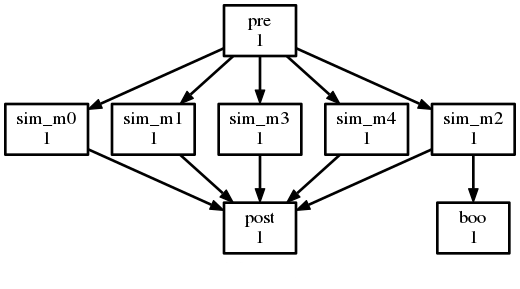
\includegraphics[width=0.5\columnwidth]{resources/jinja2-param.png}
\end{center}

\begin{shaded*}
\textbf{Tutorial}: \url{http://metomi.github.io/rose/doc/rose-rug-advanced-tutorials-jinja2.html}
\end{shaded*}

\subsection{Parameterized Tasks}

Since 6.11.0, parameter expansion can be used instead of messy Jinja2 loops
to generate tasks. Here is the parameterized task version of the
small Jinja2 example just above:

\begin{lstlisting}
[cylc]
    [[parameters]]
        m = 0..4
[scheduling]
    [[dependencies]]
        graph = """pre => sim<m> => post
                     sim<m=2> => boo"""
[runtime]
    [[sim<m>]]
        script = echo "I'm member $CYLC_TASK_PARAM_m"
    [[boo]]
        script = echo "BOO!"
\end{lstlisting}

This produces exactly the same result as the Jinja2 version, but it is much
clearer. Multiple parameters can be used at once, instead of nested Jinja2
loops.  For more on this topic see the Cylc User Guide.


\subsection{Cylc Broadcast}

\lstinline[language=bash]{cylc broadcast} is a command line utility that can
be used to change any setting contained within the \lstinline{[runtime]}
section of a suite.rc file whilst the suite is running.

\paragraph*{Example} The following line of bash script will set the remote
host for the task \lstinline{task_name}.

\begin{lstlisting}[language=bash]
$ cylc broadcast <suite_name> -n <task_name> -s [remote]host=<host_name>
\end{lstlisting}

\begin{shaded*}
\textbf{Tutorial}: \url{http://metomi.github.io/rose/doc/rose-rug-advanced-tutorials-broadcast.html}
\end{shaded*}

\subsection{Suicide Triggers}

Suicide triggers can be used to remove tasks from a suite's graph during
runtime.

\paragraph*{Example}

The task \lstinline{recover_from_failure} will be removed from the graph if
the task \lstinline{task} succeeds.

\begin{lstlisting}
[scheduling]
    [[dependencies]]
        graph = """
            task:fail => recover_from_failure  # Run recover_from_failure if
                                               # task fails.
            task => !recover_from_failure      # Don't run if task succeeds.
        """
\end{lstlisting}

\begin{shaded*}
\textbf{Tutorial}: \url{http://metomi.github.io/rose/doc/rose-rug-advanced-tutorials-suicide.html}
\end{shaded*}

\subsection{Queues}

Queues can be used to limit the number of certain tasks that are submitted or
run at any given time.

\paragraph*{Example}

In this example all \lstinline{foo}, \lstinline{bar} and \lstinline{baz} tasks
will go to the \lstinline{task_queue} queue. This queue will only allow two
tasks to run at a time.

\begin{lstlisting}
[scheduling]
    [[queues]]
        [[[task_queue]]]
            limit = 2
            members = foo, bar, baz
\end{lstlisting}

\begin{shaded*}
\textbf{Tutorial}: \url{http://metomi.github.io/rose/doc/rose-rug-advanced-tutorials-queues.html}
\end{shaded*}

\subsection{Clock Triggered Tasks}
\label{Clock Triggered Tasks}

Sometimes tasks should wait until a certain time before running, in cylc this
is possible using ''clock triggering``.

% TODO - describe as "real date-time dependencies"?

- see \ref{Clock Triggered Tasks}) 
\paragraph*{Example} $ $

\begin{lstlisting}
[scheduling]
    [[dependencies]]
        [[[T00]]]
            graph = daily_task
    [[special tasks]]
        clock-triggered = daily_task(PT0H)  # Run daily_task with 0 hours
                                            # offset from the cycle point.
\end{lstlisting}

\begin{shaded*}
\textbf{Tutorial}: \url{http://metomi.github.io/rose/doc/rose-rug-advanced-tutorials-clock-triggered.html}.
\end{shaded*}

